% Generated by benchmarks/src/utils/make_breakeven_figure.py -- do not hand-edit.
\definecolor{brk0}{HTML}{2A78D6}
\definecolor{brk1}{HTML}{EB6834}
\definecolor{brk2}{HTML}{1BAF7A}
\definecolor{brk3}{HTML}{EDA100}
\definecolor{brk4}{HTML}{E87BA4}
\definecolor{brk5}{HTML}{008300}
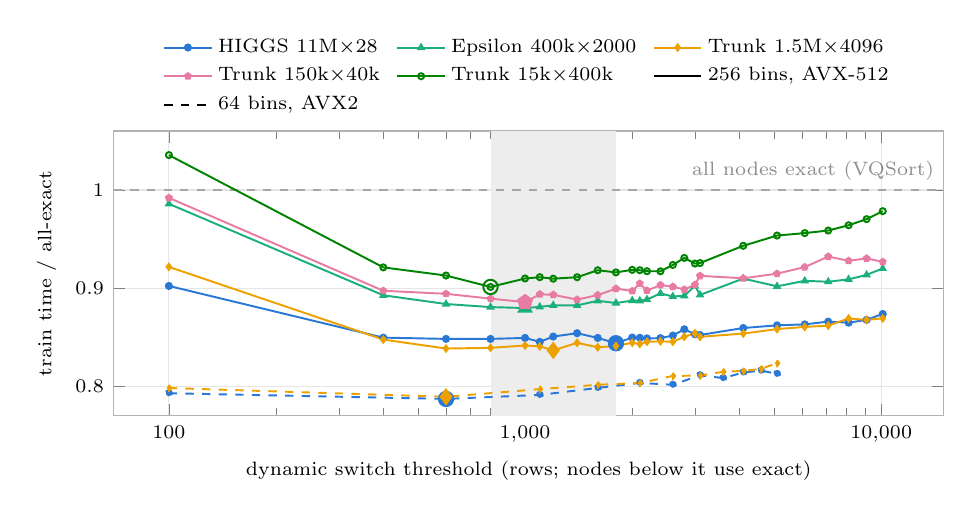
\begin{tikzpicture}
\begin{axis}[width=\linewidth, height=5.2cm, xmode=log, xmin=70, xmax=15000,
  ymin=0.77, ymax=1.06, xtick={100,1000,10000}, log ticks with fixed point,
  xlabel={dynamic switch threshold (rows; nodes below it use exact)},
  ylabel={train time / all-exact}, tick label style={font=\scriptsize},
  label style={font=\scriptsize}, grid=major, grid style={gray!20}, axis line style={gray!60},
  every axis plot/.append style={line width=0.7pt, mark size=1.1pt},
  legend style={font=\scriptsize, draw=none, fill=none, at={(0.5,1.02)}, anchor=south, legend columns=3,
    /tikz/every even column/.append style={column sep=4pt}}, legend cell align=left,
  scaled y ticks=false, yticklabel style={/pgf/number format/fixed, /pgf/number format/precision=2}]
\fill[gray!14] (axis cs:800,0.77) rectangle (axis cs:1800,1.06);
\addplot[gray!70, dashed, line width=0.6pt, forget plot] coordinates {(70,1) (15000,1)};
\node[font=\scriptsize, gray!90, anchor=south east] at (axis cs:15000,1) {all nodes exact (VQSort)};
\addplot[color=brk0, mark=*, solid] coordinates {(100,0.9023) (400,0.8497) (600,0.8484) (800,0.8484) (1000,0.8494) (1100,0.8454) (1200,0.8508) (1400,0.8542) (1600,0.8494) (1800,0.8440) (2000,0.8498) (2100,0.8495) (2200,0.8489) (2400,0.8492) (2600,0.8518) (2800,0.8582) (3000,0.8531) (3100,0.8524) (4100,0.8595) (5100,0.8622) (6100,0.8632) (7100,0.8660) (8100,0.8649) (9100,0.8678) (10100,0.8738)};
\addlegendentry{HIGGS 11M$\times$28}
\addplot[color=brk0, mark=*, mark size=2.6pt, only marks, forget plot] coordinates {(1800,0.8440)};
\addplot[color=brk2, mark=triangle*, solid] coordinates {(100,0.9859) (400,0.8928) (600,0.8839) (800,0.8808) (1000,0.8798) (1100,0.8810) (1200,0.8826) (1400,0.8825) (1600,0.8872) (1800,0.8849) (2000,0.8874) (2100,0.8872) (2200,0.8885) (2400,0.8947) (2600,0.8916) (2800,0.8923) (3000,0.9024) (3100,0.8932) (4100,0.9098) (5100,0.9019) (6100,0.9075) (7100,0.9066) (8100,0.9090) (9100,0.9136) (10100,0.9201)};
\addlegendentry{Epsilon 400k$\times$2000}
\addplot[color=brk2, mark=triangle*, mark size=2.6pt, only marks, forget plot] coordinates {(1000,0.8798)};
\addplot[color=brk3, mark=diamond*, solid] coordinates {(100,0.9217) (400,0.8477) (600,0.8386) (800,0.8393) (1000,0.8417) (1100,0.8408) (1200,0.8367) (1400,0.8444) (1600,0.8399) (1800,0.8412) (2000,0.8445) (2100,0.8432) (2200,0.8455) (2400,0.8459) (2600,0.8455) (2800,0.8506) (3000,0.8541) (3100,0.8505) (4100,0.8538) (5100,0.8584) (6100,0.8606) (7100,0.8619) (8100,0.8692) (9100,0.8678) (10100,0.8693)};
\addlegendentry{Trunk 1.5M$\times$4096}
\addplot[color=brk3, mark=diamond*, mark size=2.6pt, only marks, forget plot] coordinates {(1200,0.8367)};
\addplot[color=brk4, mark=pentagon*, solid] coordinates {(100,0.9920) (400,0.8974) (600,0.8943) (800,0.8894) (1000,0.8858) (1100,0.8938) (1200,0.8933) (1400,0.8884) (1600,0.8930) (1800,0.8996) (2000,0.8971) (2100,0.9048) (2200,0.8976) (2400,0.9032) (2600,0.9015) (2800,0.8987) (3000,0.9035) (3100,0.9126) (4100,0.9101) (5100,0.9148) (6100,0.9215) (7100,0.9322) (8100,0.9279) (9100,0.9303) (10100,0.9268)};
\addlegendentry{Trunk 150k$\times$40k}
\addplot[color=brk4, mark=pentagon*, mark size=2.6pt, only marks, forget plot] coordinates {(1000,0.8858)};
\addplot[color=brk5, mark=o, solid] coordinates {(100,1.0355) (400,0.9212) (600,0.9129) (800,0.9013) (1000,0.9099) (1100,0.9112) (1200,0.9097) (1400,0.9112) (1600,0.9183) (1800,0.9161) (2000,0.9187) (2100,0.9183) (2200,0.9173) (2400,0.9172) (2600,0.9237) (2800,0.9308) (3000,0.9251) (3100,0.9256) (4100,0.9432) (5100,0.9536) (6100,0.9561) (7100,0.9587) (8100,0.9641) (9100,0.9703) (10100,0.9784)};
\addlegendentry{Trunk 15k$\times$400k}
\addplot[color=brk5, mark=o, mark size=2.6pt, only marks, forget plot] coordinates {(800,0.9013)};
\addplot[color=brk0, mark=*, dashed, forget plot] coordinates {(100,0.7931) (600,0.7873) (1100,0.7914) (1600,0.7985) (2100,0.8036) (2600,0.8017) (3100,0.8114) (3600,0.8085) (4100,0.8142) (4600,0.8161) (5100,0.8128)};
\addplot[color=brk0, mark=*, mark size=2.6pt, only marks, forget plot] coordinates {(600,0.7873)};
\addplot[color=brk3, mark=diamond*, dashed, forget plot] coordinates {(100,0.7984) (600,0.7895) (1100,0.7973) (1600,0.8017) (2100,0.8035) (2600,0.8107) (3100,0.8111) (3600,0.8150) (4100,0.8158) (4600,0.8180) (5100,0.8237)};
\addplot[color=brk3, mark=diamond*, mark size=2.6pt, only marks, forget plot] coordinates {(600,0.7895)};
\addlegendimage{color=black, solid, line width=0.7pt, mark=none}
\addlegendentry{256 bins, AVX-512}
\addlegendimage{color=black, dashed, line width=0.7pt, mark=none}
\addlegendentry{64 bins, AVX2}
\end{axis}
\end{tikzpicture}
